% Use only LaTeX2e, calling the article.cls class and 12-point type.

\documentclass[12pt]{article}

% Users of the {thebibliography} environment or BibTeX should use the
% scicite.sty package, downloadable from *Science* at
% www.sciencemag.org/about/authors/prep/TeX_help/ .
% This package should properly format in-text
% reference calls and reference-list numbers.



\usepackage[pdftex]{graphicx}

\usepackage[labelfont=bf]{caption}

\usepackage{indentfirst}

\usepackage{scicite}

% Use times if you have the font installed; otherwise, comment out the
% following line.

\usepackage{times}

% The preamble here sets up a lot of new/revised commands and
% environments.  It's annoying, but please do *not* try to strip these
% out into a separate .sty file (which could lead to the loss of some
% information when we convert the file to other formats).  Instead, keep
% them in the preamble of your main LaTeX source file.

% The following parameters seem to provide a reasonable page setup.

\topmargin 0.0cm
\oddsidemargin 0.2cm
\textwidth 16cm 
\textheight 21cm
\footskip 1.0cm

%The next command sets up an environment for the abstract to your paper.

\newenvironment{sciabstract}{%
\begin{quote} \bf}
{\end{quote}}


% Include your paper's title here

\title{Critical brain: the statistical physics of neural systems} 


% Place the author information here.  Please hand-code the contact
% information and notecalls; do *not* use \footnote commands.  Let the
% author contact information appear immediately below the author names
% as shown.  We would also prefer that you don't change the type-size
% settings shown here.

\author
{Kevin Gilmore}

%%%%%%%%%%%%%%%%% END OF PREAMBLE %%%%%%%%%%%%%%%%



\begin{document} 

% Double-space the manuscript.

\baselineskip24pt

% Make the title.

\maketitle 

% Place your abstract within the special {sciabstract} environment.

\begin{sciabstract}
No comprehensive model of the brain exists. Recent results in experimental and theoretical neuroscience indicate the brain may be operating as though at a critical point in a continuous phase transition. Methods in statistical physics are able to shed some light on this phenomena. As a result, models abstracted of biological details that consider networks of excitable elements at criticality capture the emergent, macroscopic behavior of the brain.
\end{sciabstract}

\section*{Introduction}

The human brain is amazingly complex. Comprised of tens of billions of neurons with a hundred trillion connecting synapses, it is no wonder it remains so poorly understood. From this immensely complex network of interacting elements arise collective dynamics, which neuroscience has only recently turned its focus to. However, the study of collective phenomena is well known to physics. Statistical mechanics uses probability theory to ascertain the collective behavior of systems made up of very large numbers of constituents, thereby connecting the microscopic to the macroscopic. As a result, some theorized the brain could operate in a regime characterized by statistical mechanics as a continuous phase transition\cite{Bak1987a}. Significant credence was given to this theory with the first experimental evidence that neuronal networks exhibit avalanches reminiscent of a system operating at criticality, i.e. at the critical point in a continuous phase transition \cite{Beggs2003b}.

\paragraph*{Motivation} Understanding the underlying mechanism by which the brain adaptively produces a broad range of behaviors is a fundamental problem in neuroscience. Indeed, the mechanism responsible for the emergence of behavior from simple excitable elements (neurons) interacting via electrochemical impulses is of ultimate importance in understanding intelligent life. Naturally, a subject of such fundamental interest and great complexity, but which can nonetheless be modeled simply, attracts physicists. 

Of course, mere interest does not suffice. Does physics really have something to contribute to the field of neuroscience in the context of neuronal networks? In the course of this paper, I will argue that it does. The facts that networks of excitable elements operating at criticality benefit from maximal dynamic range \cite{Kinouchi2006b,Shew2009b} and information capacity\cite{Shew2011a} show that a statistical mechanical approach to understanding neuronal networks, and thus the brain, has real functional yield.

\paragraph*{Overview} In this paper I will discuss recent work in the emerging subfield of criticality in neural systems. Work in this field combines experimental neuroscience, nonlinear dynamics, complex systems, and graph theory in the context of statistical physics. To understand the human brain, and thus our behavior and cognition, necessitates the elucidation of the patterns of spatiotemporal brain activity that arise out of collective neural dynamics. To this end, the tools of statistical mechanics, and in particular those dealing with critical phenomena, may be of great use.

The structure of the paper is as follows. First, I review relevant background information from the physics of phase transitions as well as network theory. Then, I explain how a simple microscopic model - the Ising model - reproduces macroscopic network behavior observed in the brain. Next is a description of the experimental observation of neuronal avalanches following a power-law scaling, which is the main evidence of the brain operating at a critical point in a continuous phase transition. Finally, I discuss how this model explains the brain's large information capacity and dynamic range.

\section*{Physics of phase transitions and critical phenomena}

Statistical physics has had great success in explaining the emergence of macroscopic thermodynamic behavior from underlying microscopic interactions. An emergent phenomena is a macroscopic one that can be explained simply, though it arises out of complicated microscopic interactions. Many interdisciplinary fields have attempted to make use of statistical mechanics to explain phenomena arising out of complicated dynamics. In the context of the brain, complicated neuronal interactions lead to conscious behavior. Perhaps the emergence of psychological phenomena may be simply modeled by the physics of phase transitions.

A phase transition is a qualitative change in the macroscopic properties of a substance. Typically, this change occurs as a function of an external parameter, such as temperature. To quantify a phase transition, it is useful to look for a physical property that distinguishes between the two phases. Such an observable is called an order parameter. For the liquid-solid water transition, the density (or volume) is an example of an order parameter. In this case, the density changes discontinuously at the phase transition. There is an abrupt change from ice to water. Such phase transitions are called discontinuous phase transitions.

Continuous phase transitions occur when the order parameter changes continuously across the transition from one phase to another. The critical point in a continuous phase transition is the point at which certain physical properties of the system in question are singular and the system itself is in some sense teetering between two phases, between two qualitatively different states such as order and disorder. These physical properties are known as susceptibilities, and are indicative of the response of the system to external perturbations. Divergent susceptibility and infinite correlation length are two of the defining characterizations of continuous phase transitions.

The 2D Ising model is one of the simplest models demonstrating a phase transition, illustrated in Figure \ref{Figure::Ising model criticality}. The Ising model is a mathematical model consisting of interacting spins $s$ on a lattice. The spins take values of +1 or -1 and are coupled together through an interaction strength parameter $J$. The Hamiltonian for the Ising model is

\begin{equation}
\mathcal{H} = - \sum_{ij}Js_{i}s_{j} - H\sum_{i}s_{i},
\end{equation}

where the sum $(ij)$ is over all pairs of nearest-neighbor sites. In the context of magnetism, $H$ is the external field and the sum $M=\sum\limits_{i} s_{i}$ is the magnetization. In the case of no external field, as its temperature is increased a magnet may undergo a second order phase transition from ferromagnetic to paramagnetic. As the system approaches a critical temperature the magnetization vanishes continuously. At the critical temperature, the magnetization fluctuates wildly corresponding to neither an ordered ferromagnetic nor disordered paramagnetic state.

Two main features of continuous phase transitions are scale-invariance and universality. That a phase transition is scale-invariant means fluctuations occur at all length scales, and so such systems are statistically invariant under changes in length scale. Universality signifies a lack of dependence on microscopic properties near the critical point. As a result, widely different microscopic systems can display the same macroscopic behavior at a phase transition. The same scale-invariant theory can be used to describe many different systems. Properties such as susceptibility, specific heat, and correlation lengths have power law singularities at the critical point. The critical exponents corresponding to these power laws  may be shared between seemingly disparate systems such as ferromagnets and liquid-gas systems, which as a result may both be modeled by the Ising model. Most relevant for the discussion to follow in this paper is the power-law decay of correlations that occurs near the critical point. These features of continuous phase transitions at the critical point are collectively referred to as critical phenomena.

In much the same way ferromagnetism emerges from the interactions of spins, the mind may be an emergent property of neuronal interactions. 

\begin{figure}      
  \begin{center}    
 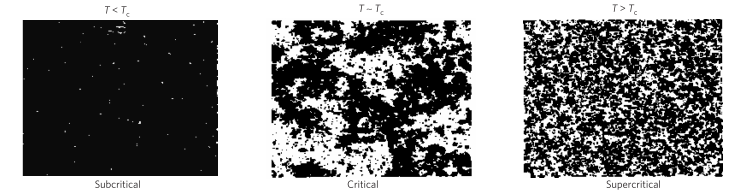
\includegraphics[width=1\textwidth]{Isingchialvo}    
    \caption{\textbf{2D Ising model \cite{Chialvo2010a}.} Snapshots of spin configurations demonstrating a continuous phase transition. Here, the external field is zero and the temperature is being tuned across its critical value. White pixels correspond to spin up (+1), while black is spin down (-1). In the subcritical and supercritical states homogenous order and disorder reign, respectively. At the critical temperature fluctuations occur on all length scales due to highly correlated sections.}  
   \label{Figure::Ising model criticality}   
  \end{center}     
   \end{figure}
 
\paragraph*{Avalanches}

A number of physical systems built out of interacting constituents are characterized by impulsive avalanches of activity. These avalanches may vary greatly in size, and in some cases the system exhibits avalanches of all scales. Systems displaying such scale invariance may be studied with the same tools as those in the study of continuous phase transitions. At criticality, these avalanches span the size of the system. The number of avalanches $D$ of a size $s$ follows a power law $ D(s) \sim s^{-\tau} $ over several orders of magnitude. This power law behavior results in a distinctive probability distribution in size. Earthquakes are an example of one such phenomena\cite{Sethna2011a}. An earthquake is caused by the grinding of two sides of a fault in a stick-slip type motion. The faults remain stuck for small applied stresses, and with strong stresses the faults simply slide by each other. However, at the transition between these two qualitatively different behaviors is a critical regime where earthquakes of all sizes are seen. In the Ising model for magnetism, avalanches appear as fluctuations in the magnetization due to the propagation of spin flips. 

A system exhibiting scale invariance in the form of avalanches of activity that follow power law probability distributions in size may be modeled as a system at the critical point in a continuous phase transition. As will be seen, networks of neurons - and thus the brain - are one such system.

\section*{Networks and branching processes}

Often, complex systems comprised of numerous interacting parts - such as the brain - are modeled as networks. Networks, individuals and the complicated interconnections between them, are represented mathematically as collections of nodes with connecting links. Structural properties of a network's topology may be analyzed to give insight into the workings of the network. One such property is the degree distribution. The degree of a node is the number of connections it has to other nodes. So, the degree distribution is the probability distribution of all the degrees of the nodes in the network. 

The propagation of activity in networks is often modeled with branching processes. Branching processes were originally studied in the context of the survival of aristocratic family names in the Victorian era\cite{Watson2014}, and more recently in understanding the propagation of disease. An excited node branches to other nodes with some probability. In the case of a critical branching process, the sum of the probabilities of the nodes excited from one generation to the next is equal to one. This sum is known as the branching ratio. The propagation of excitations in a branching process behaves as the avalanches previously described. In the critical regime, both the size $s$ and duration $t$ of the avalanches follow power laws $ D(s) \sim s^{-3/2} $ and $ D(t) \sim t^{-2} $, respectively \cite{Larremore2014}. Should the average number of active nodes increase (decrease), the process is dubbed supercritical (subcritical) - as illustrated in Figure \ref{Figure::Critical Branching Process}. 

\begin{figure}      
  \begin{center}    
 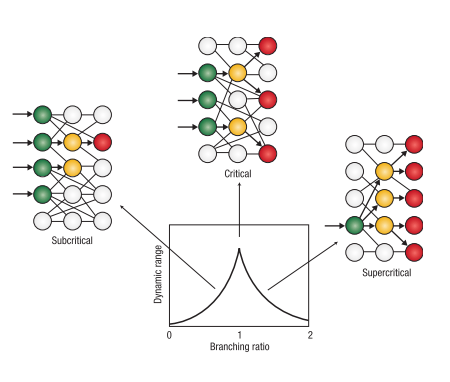
\includegraphics[width=.7\textwidth]{Branchingprocesschialvo}    
    \caption{\textbf{Branching processes \cite{Chialvo2006a}.} Subcritical branching processes quickly die out, while the system is saturated in the supercritical regime. Only in the critical state with $\sigma = 1$ is the input activity maintained, on average. At criticality, the system is sensitive to both small and large pertubations, thus maximizing its dynamic range.}
   \label{Figure::Critical Branching Process}   
  \end{center}     
   \end{figure}

\section*{The Ising model and the brain}
Certain macroscopic phenomenological features of the brain can be replicated by using the 2D Ising model as minimal model for brain activity \cite{Fraiman2009a}. Brain functional magnetic resonance imaging (fMRI) data and a 2D Ising model simulation were transformed into networks and their degree distributions analyzed. Correlations between sites in both were computed, with links between sites defined whenever the correlation is greater than or equal to a given threshold. By setting this threshold, the average degree of the network may be regulated. The degree distributions at particular average degrees for both the Ising model at criticality and brain FMRI data display remarkable similarity (see Figure \ref{Figure::Ising model and the brain at criticality}). Despite the simplicity of the Ising model and its complete lack of any neural details, the macroscopic, phenomenological behavior of the brain can still be replicated. This finding lends support to the idea that the brain operates in a critical regime where its microscopic details are not relevant to the emergent macroscopic behavior and network dynamics.

\begin{figure}      
  \begin{center}    
 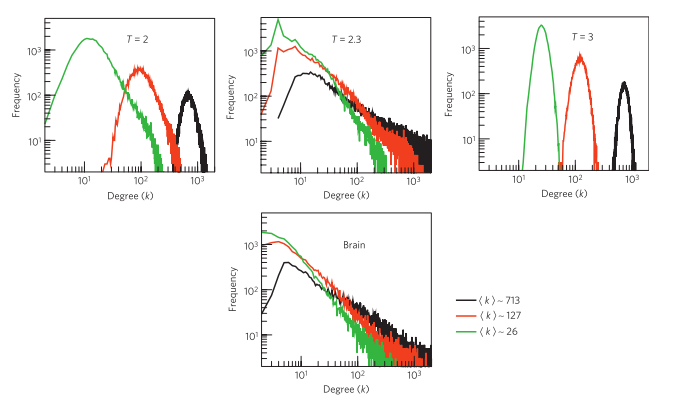
\includegraphics[width=.8\textwidth]{isinglikedynamicschialvo}    
    \caption{\textbf{Ising-like dynamics of the brain \cite{Fraiman2009a}.} Degree distributions from fMRI brain data (bottom) and Ising model (top) at temperatures corresponding to subcritical ($T=2$), critical ($T=2.3$), and supercritical ($T=3$). Black, red, and green curves correspond to average network degrees of 713, 127, and 26, respectively.}
   \label{Figure::Ising model and the brain at criticality}   
  \end{center}     
   \end{figure}
  
\section*{Neuronal avalanches}

In general, complex systems, such as networks of neurons, are characterized by two phases: a noisy, chaotic state with very weak interactions and a frozen, static state with very strong interactions - with a mediating critical junction. The brain must maintain some order to ensure consistent behavioral responses to particular stimuli as well as some degree of disorder to enable flexibility in the form of adaptive changes to a dynamic environment, implying it operates at criticality \cite{Bak1987a}. Experiments such as the previously discussed Ising model comparison lend further weight to this notion. Experimental demonstration of neuronal avalanches gives further, more robust evidence of the brain functioning at a critical point.

In 2003, the first experimental evidence that neuronal activity does involve neuronal avalanches - impulsive propagation of activity from individual neurons firing and triggering subsequent neurons to fire - was published\cite{Beggs2003b}. By studying the propagation of spontaneous neuronal activity in slices of rat cortex on multielectrode arrays, Beggs and Plenz observed avalanches of signal with size distribution $ D(s) \sim s^{-3/2} $ (Figure \ref{Figure::Neuronal Avalanches}). Avalanches occur up to the size of the system (the number of electrodes), which is consistent with avalanches occurring at a critical point. Over 2 orders of magnitude the distribution is a power law with exponent -3/2. In addition, the branching parameter, i.e. the number of neurons excited step-by-step during the avalanche, is about 1. Neuronal avalanches in several systems follow power laws just as would be expected from a critical branching process (Figure \ref{Figure::Neuronal avalanches in vitro and in vivo}).
 
\begin{figure}      
  \begin{center}    
 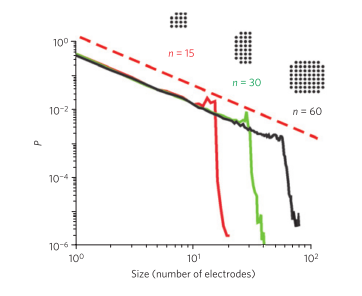
\includegraphics[width=.6\textwidth]{originalavalancheplenz}    
    \caption{\textbf{Size distribution of neuronal avalanches} in cortical cultured networks follows a power law with exponent of approximately -3/2 (dashed line) \cite{Beggs2003b}. Insets indicate number of electrodes, and thus network size. Avalanches occur up to system size.}
   \label{Figure::Neuronal Avalanches}   
  \end{center}     
   \end{figure}
   
\begin{figure}      
  \begin{center}    
 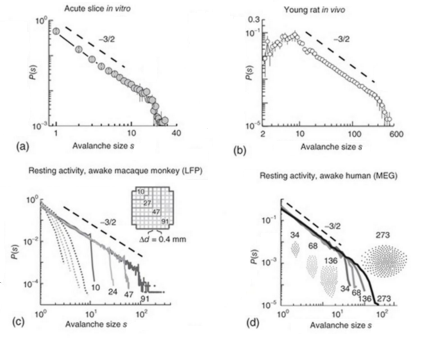
\includegraphics[width=1\textwidth]{avalanchesplenzbook2}    
    \caption{\textbf{Comparison of neuronal avalanches in several systems \cite{Plenz2014}.} (a) Neuronal avalanches in rat cortex slice \textit{in vitro}. (b) Neuronal avalanches in rat \textit{in vivo}. (c) Neuronal avalanches in awake macaque monkey. Cutoff corresponds to area of array i.e. number of electrodes. (d) Resting magnetoencephalography (MEG) of the human brain demonstrating neuronal avalanches. Sensor array size noted in inset and by grayscale and numbers on plot.}
   \label{Figure::Neuronal avalanches in vitro and in vivo}   
  \end{center}     
   \end{figure}

Experimental evidence points towards networks of neurons operating in a critical regime characterized by power laws, but simply observing a trend in data that follows a power law does not establish the presence of critical phenomena. Some physical parameters must be shown to pass through a singularity, and the generative mechanism of the phenomena should be theoretically described. In addition, the use of the concept of criticality ought to be applied only if it yields some insight. Crucially, if the critical brain story is to be legitimized there must be a functional purpose for this supposed phenomena. 
      
\section*{The brain as an information processor}

The brain is an information processor. Any theory purported to describe neuronal networks should account for what we know about the information processing capabilities of the brain. The theory of criticality in networks provides something novel. Through both theoretical models and experimental findings, it has been shown that networks of neurons achieve maximal information capacity and dynamic range at criticality. Thus, there is a functional benefit to maintaining a critical state in the brain.
   
The intensity of human-detectable physical stimuli, such as light and sound, varies by several orders of magnitude. For hearing the dynamic range is on the order of 140 dB, for sight it is 90 dB. This very large dynamic range must be accounted for in the model. Since single neurons respond in a linear, saturating way with a limited range, the broad dynamic range must be a collective phenomena. Kinouchi and Copelli demonstrated computationally(see Figure \ref{Figure::Dynamic Range Theory}) that a network of excitable elements, such as a neuronal network, has its dynamic range and sensitivity maximized at its critical point during a non-equilibrium phase transition\cite{Kinouchi2006b}. This finding is consistent with and lends further credence to the brain operating at criticality. The dynamic range is calculated from the $10\%-90\%$ response interval and is seen to be maximized at the critical branching ratio. In the subcritical regime, the dynamic range increases with the branching ratio. In the supercritical regime, the dynamic range decreases with the branching ratio \cite{Larremore2011a, Larremore2012a}.

\begin{figure}      
  \begin{center}    
 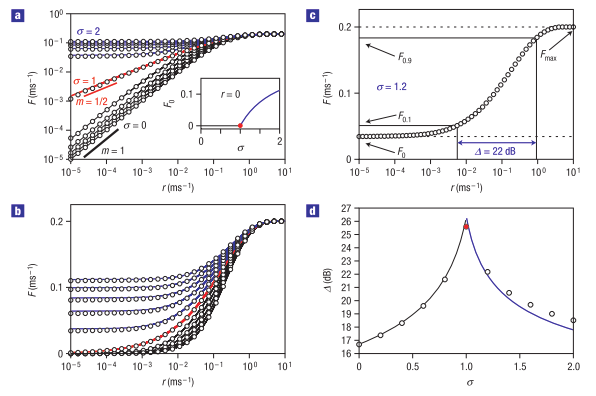
\includegraphics[width=1\textwidth]{dynamicrangetheorycopelli}    
    \caption{\textbf{Simulations of response curves and dynamic range} for generic model of network of interacting, excitable elements \cite{Kinouchi2006b}. \textbf{(a, b)} Average activity $F$ (i.e. number of excited elements) versus stimulus rate $r$ with branching parameters from $\sigma = 0$ to 2 in intervals of 0.2. The data is represented logarithmic and linear scales in \textbf{(a)} and \textbf{(b)}, respectively. \textbf{(c)} Response curve for $\sigma = 1.2$ with dynamic range $\Delta$ from $10\%$ to $90\%$ of saturated response. \textbf{(d)} Dynamic range versus branching ratio. Optimization occurs at the critical point $\sigma = 1$.}
   \label{Figure::Dynamic Range Theory}   
  \end{center}     
   \end{figure}

The ability of a neuronal network to process information is determined by the neural activity it produces. Activity patterns in cortex cultures, anesthetized rats, and awake monkeys were measured to quantify their dynamic range (Figure \ref{Figure::Dynamic Range Experiment}) and information capacity (Figure \ref{Figure::Entropy / information maximized experimental}). Experiments have demonstrated that networks generating neuronal avalanches benefit from maximized dynamic range\cite{Shew2009b}. By measuring the responses to a range of stimuli amplitudes, the dynamic range was computed by way of the same response interval as in the theoretical approach.
   
In a similar study, the information capacity was measured and found to be maximized at a balanced ratio corresponding to the emergence of neuronal avalanches by changing the ratio of excitation to inhibition in these subjects by way of excitory and inhibitory drugs \cite{Shew2011a}. Multielectrode arrays comprised of an 8x8 grid of electrodes were used to record events, with 1 bit assigned to each electrode. Thus, different activity levels correspond to distinct binary patterns. Information capacity can be quantified by calculating the Shannon entropy, defined as

\begin{equation}
H = - \sum^{n}_{i=1}p_{i}\log_{2}p_{i},
\end{equation}

\noindent where n is the number of binary patterns and $ p_{i} $ is the probability that a particular pattern $i$ occurs. The agreement between experimental findings and theoretical models supports the theory of neuronal networks operating at criticality and suggests that in networks with balanced excitation and inhibition maximal information processing capabilities arise as a result of criticality. 

\begin{figure}      
  \begin{center}    
 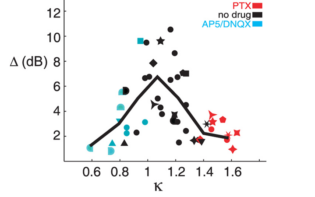
\includegraphics[width=.6\textwidth]{dynamicrangeexpplenz}    
    \caption{\textbf{Dynamic range \cite{Shew2009b}.} Experimental data taken with no administered drug (black) a drug that reduces inhibition (red) and a drug that reduces excitation (blue). Dynamic range peaks near $\kappa = 1$. $\kappa$ is a measure of the difference between experimental results and theoretical reference and is nearly linearly related to the branching parameter $\sigma$. $\kappa \cong 1$ corresponds to the critical regime where $\sigma = 1$. Black line indicates binned average of points. Shared symbol shape indicates paired measurements: no drug condition measured just before the drug condition. Circles represent unpaired measurements.}
    
   \label{Figure::Dynamic Range Experiment}   
  \end{center}     
   \end{figure}
  
\begin{figure}      
  \begin{center}    
 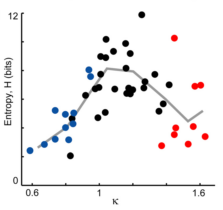
\includegraphics[width=.50\textwidth]{entropyplenz}    
    \caption{\textbf{Information capacity \cite{Shew2011a}.} Experimental data taken with same drug-color scheme as previous figure. Information entropy is maximized around $\kappa = 1$. Black line indicates binned average of points.}
   \label{Figure::Entropy / information maximized experimental}   
  \end{center}     
   \end{figure}

To summarize these experimental and theoretical findings, neuronal avalanches with power law distributions in size and duration were observed and found to maximize neuronal information processing in the form of dynamic range and information capacity (information entropy). These findings are consistent with the theory that neuronal networks operate at criticality. 



\section*{Criticisms} The search for qualitative links between empirical data from complex phenomena and simple models should be done cautiously and viewed with some skepticism. In particular, though the rule of thumb for a purported power law says the relationship should hold over two orders of magnitude \cite{Sethna2011a}, many published results do not fit this criterion. Rather than following a particular power law, many of these data sets are merely heavy-tailed. However, much of the data concerning neuronal avalanches does span at least two orders of magnitude, or is cut off by the experimental limitation of electrode size. Even if the statistics have been properly dealt with, has anything been gained in borrowing the language of critical phenomena? In the context of criticality in neural systems, the answer is - though not unequivocally - yes. Though ``imbuing them with a vague and mistakenly mystical sense of universality'' \cite{Stumpf2012a} is a mistake, neuronal networks are better understood as a result of the application of the concepts of statistical mechanics and critical phenomena. 

There is real functional benefit and thus reason for neuronal networks to operate at criticality: their dynamic range and information capacity is maximized. Thus there is biologically and evolutionarily motivated physical insight into the workings of the brain to be found in the study of criticality in neural systems.

Even if empirical data supports modeling neuronal networks as operating at criticality and doing so has explanatory power, it is not clear how this could be the case. Typically, phase transitions occur as a result of the fine-tuning of an external parameter, such as temperature. Clearly there is no external mechanism doing this fine-tuning in the case of the brain, which would require somehow perpetually holding the brain in a critical regime. 

An interesting exception to this fine-tuning requirement is a dynamical system whose critical point acts as an attractor. In such a system, no fine tuning is necessary and despite starting far from equilibrium the critical regime may be reached. Bak's sandpile model\cite{Bak1987a} was the first example of a dynamical system displaying such self-organized criticality. Grains of sand are gradually and randomly added to a pile. As the pile of sand grows, if the slope becomes too large the pile will collapse via avalanche. The cycle of growth and collapse continues until the slope reaches a point wherein the pile is barely stable to small perturbations. Apparently this system is attracted to its critical point with no tuning of an external parameter - unlike more typical examples of critical phenomena. Such a system is said to exhibit self-organized criticality.
   
Though the generative mechanism for self-organized criticality in the brain is not known (nor within the scope of this paper), several theoretical models involving dynamical synapses have been proposed and comfirmed to exhibit the desired effects \cite{Levina2007a, Levina2009a, Bornholdt2003a, Rybarsch2014a}. It seems plausible that the brain could exhibit self-organized criticality, thereby removing the need for any fine-tuning.

\section*{Conclusions}

To conclude, neuronal avalanches following power law relationships in probability distribution of size and duration have been observed and the consequences discussed. Theoretical models and empirical data suggest that these avalanches occur in a critical regime and may be qualitatively and quantitatively understood through the lens of the critical phenomena of statistical physics. In addition, theoretical and experimental results indicate that networks of neurons, and indeed animal and human brains, benefit from maximized dynamic range and information capacity as a result of operating at criticality. Further, qualitative links to the Ising model more firmly establish the role of critical phenomena in neural systems. The significance of these findings is to establish an interdisciplinary field merging complex systems, neuroscience, mathematics, and physics. This emerging field of criticality in neural systems is a promising endeavor which has already yielded great insights into the fundamental workings of the brain. It seems physics may yet have a great deal to contribute to one of the greatest known mysteries: the human brain. 

\bibliographystyle{ieeetr}

\bibliography{Bib}

\end{document}
